 \documentclass[11pt, oneside]{article}   	% use "amsart" instead of "article" for AMSLaTeX format
\usepackage{geometry}                		% See geometry.pdf to learn the layout options. There are lots.
\geometry{letterpaper}                   		% ... or a4paper or a5paper or ... 
%\geometry{landscape}                		% Activate for for rotated page geometry
%\usepackage[parfill]{parskip}    		% Activate to begin paragraphs with an empty line rather than an indent
\usepackage{graphicx}				% Use pdf, png, jpg, or eps§ with pdflatex; use eps in DVI mode
								% TeX will automatically convert eps --> pdf in pdflatex		
\usepackage{amssymb}
\usepackage{amsmath}
\usepackage{parskip}
\usepackage{color}
\usepackage{hyperref}

\title{Cauchy's residue theorem}
%\author{The Author}
%\section{}
%\subsection*{}
\date{}							% Activate to display a given date or no date

\graphicspath{{/Users/telliott_admin/Dropbox/Tex/png/}}
% \begin{center} 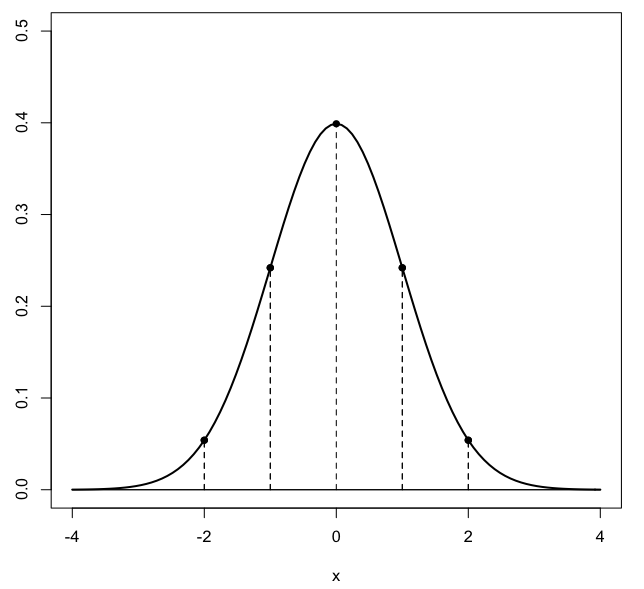
\includegraphics [scale=0.4] {gauss3.png} \end{center}
\begin{document}
\maketitle
\Large
If we can write an integral in this form:
\[ \oint_{C} \frac{f(z)}{z-z_0} \ dz \]
where $f(z)$ is analytic and defined everywhere in the domain we care about, with this composite function of course not defined at $z = z_0$, then we will show that the value of the integral is 
\[ \oint_C \frac{f(z)}{z-z_0} \ dz = 2 \pi i f(z_0) \]
This is called Cauchy's Residue Theorem, or simply Cauchy 2.

\subsection*{derivation}
Suppose $f(z)$ is analytic and defined everywhere within some region \emph{except} at a singularity, $z_0$.  For example, suppose we have
\[ \frac{f(z)}{z-z_0} \]
We integrate this function around a special closed path in the region of analyticity:
\[ \oint \frac{f(z)}{z-z_0} \ dz \]
\begin{center} 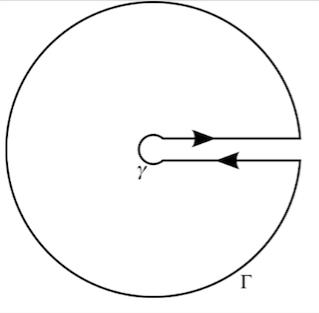
\includegraphics [scale=0.5] {keyhole.png} \end{center}
It's not labeled (I didn't draw the figure) but the singularity $z_0$ is at the center of the two concentric circles.  The "keyhole" excludes $z_0$ so $f$ is analytic everywhere in the region enclosed by the path.

Cauchy's first theorem tells us that the total integral is zero.

The straight line segments are so close to each other as to be equal, but traversed in opposite directions, so the net contribution from them is zero.

Therefore by Cauchy 1 we have that the integral around the outer ring counter-clockwise + the integral around the inner ring clockwise add up to zero.

But reversing the direction of integration on the inner ring (so both paths go in the counter-clockwise direction) changes the sign of the value, hence we have that
\[ \oint_{C \ \text{outer}} \frac{f(z)}{z-z_0} \ dz - \oint_{C \ \text{inner}} \frac{f(z)}{z-z_0} \ dz = 0 \]
and
\[ \oint_{C \ \text{outer}} \frac{f(z)}{z-z_0} \ dz = \oint_{C \ \text{inner}} \frac{f(z)}{z-z_0} \ dz \]

Notice that we haven't said anything about the radius of these rings.  

What this means is that the value of the integral around a ring enclosing a singularity is not zero, but is independent of the radius.

We can parametrize this path by realizing that each point on one of these curves is given by
\[ z = z_0 + \rho e^{i\theta}, \ \ \ 0 \le \theta \le 2 \pi \]

Since $z_0$ is a constant
\[ dz = i \rho e^{i \theta} d \theta \]
But
\[ z - z_0 = \rho e^{i\theta} \]
so, substituting for $\rho e^{i\theta}$ above we obtain
\[ dz = i(z - z_0) \ d \theta \]
and
\[ \oint \frac{f(z)}{z - z_0} \ dz = \oint f(z) \ i \ d \theta \]
\[ = i \int_0^{2\pi}  f(z) \ d \theta \]

This holds for every circular path enclosing $z_0$.  We may choose $\rho$ as small as we like, and so we choose it very small ($\rho \rightarrow 0$) so
\[ f(z) \rightarrow f(z_0) = \text{constant} \]
and since it's constant we can bring it out from under the integral sign!
\[ i \int_0^{2\pi}  f(z) \ d \theta \]
\[ = i f(z_0) \int_0^{2\pi} d \theta = 2 \pi i f(z_0) \]
Summarizing:
\[ \oint \frac{f(z)}{z - z_0} \ dz = 2 \pi i f(z_0) \]
What this means is that we can evaluate the integral in question by simply plugging in the value of the function at $z_0$ and multiplying that by $2 \pi i$.

\subsection*{examples}
Our formula is:
\[ \oint_{C} \frac{f(z)}{z-z_0} \ dz = 2 \pi i f(z_0) \]

A very simple example is:
\[ \oint_{C} \frac{1}{z} \ dz \]
Here $f(z) = 1$ and $z_0 = 0$ and the result should be
\[ I = 2 \pi i f(z_0) = 2 \pi i  \]
We computed this directly using the unit circle centered at $z = 0$.  We have that
\[ z = e^{i\theta} \]
\[ dz = i z \ d \theta \]
so
\[ \oint_{C} \frac{1}{z} \ dz = \int_0^{2 \pi}  \frac{1}{z} \ i z \ d \theta \]
\[ = \int_0^{2 \pi} i \ d \theta \]
\[ = 2 \pi i \]

\subsection*{translated from the origin}
Suppose we are interested in the value of the integral centered at a point $z_0 \ne 0$.  We consider those points $z$ in a circle constructed around $z_0$, that is
\[ z = z_0 + re^{it} \]
rearranging
\[ z - z_0 = re^{it} \]
We get the derivative of the polar form
\[ \frac{d}{dt} \ re^{it} = i re^{it}  \]
\[ = i(z-z_0) \]
Hence
\[ \int \frac{1}{(z-z_0)} \ dz  = \int \frac{1}{(z-z_0)} \ i(z - z_0) \ dt \]
\[ = 2 \pi i \]

However, we can also do this by Cauchy 2. The formula is
\[ \int \frac{f(z)}{z - z_0} \ dz = 2 \pi i \ f(z_0) \]
here the integrand is
\[ \frac{1}{(z-z_0)} \]
so $f(z)$ is just equal to $1$, and the answer is $2 \pi i$.

\subsection*{extension}
A specific extension of the Cauchy Integral formula 
\[ f(z) = \frac{1}{2 \pi i} \int_C \frac{f(w)}{w - z} \ dw \]
is
\[ f'(z) = \frac{1}{2 \pi i} \int_C \frac{f(w)}{(w - z)^2} \ dw \]
Brown and Churchill give the proof for this specific case, but not for the general one (which is also true) because it's too hard for their book:

\[ f^n(z) = \frac{n!}{2 \pi i} \int_C \frac{f(w)}{(w - z)^{n+1}} \ dw \]

However they do point out that one simple approach is to differentiate with respect to $z$ under the intnegral sig (without real justification).  That gives the result above quite simply.


\end{document}  
